\mychapter{Time Warp}

\section{Introduction}

During the course of this project there were two focus of studies on Time Warp (TW).  First off we must define what it means to be a TW system and secondly we must configure the KMC problem in such a way that it fits in with the TW algorithm.  The first study was rather simple in it's function.  However the second was much more in-depth and was the primary focus of work.

\subsection{Time Warp Algorithm: Classic}

Classically, TW is defined as a "\textit{optimistic}, object-oriented, distributed, discrete-event simulation mechanism"~\cite{obgl:tw}.  This is different then classical approaches to distributed-event simulation (DES), in that it's not conservative.  This allows TW to better exploit the "concurrency in distributed simulations"~\cite{obgl:tw}.

The distinction must be made between optimistic and conservative synchronization algorithms.  Time Warp falls into the former category, which is to execute and attempt to solve for the solution correcting errors as they occur, which is an asynchronous operation.  In a conservative algorithm, part of a solution is solved, after which any errors are corrected, ad infinitum until the correct solution for that subsection of the entire solution is correct.  Then the algorithm can move on to the next subsection.  The entire algorithm is synchronous, as all executing programs will proceed in lock-step until they arrive at the final solution.

In a TW system you have three components.  The first component is the local virtual time (LVT), which is local to each TW object, and is the method by which that object timestamps and synchronizes messages.  The LVT advances independently of each other clock, this is the asynchronous nature of the algorithm.  The system is optimistic because each TW object advances even if there is the possibility for an error in the computation.

The second component is the error correction or \textit{rollback}.  This move the simulation back in time to a point before the error occurs.  The simulation can then proceed from this point, fixing the error when it occurs.  Any computations (events) that are not performed when the error is corrected are canceled by anti-messages.

However, there is a trade-off for the optimistic nature of the algorithm.  We incur a penalty each and every time we must roll back the simulation to fix an error.  The penalty is in the cost of the the roll-back and the extempores calculations that we may have performed.

Lastly, there is the third component, the global virtual time (GVT).  This is the lowest LVT that is associated with any TW object.  The GVT is used to garbage collect out-of-date objects, messages, and roll-back checkpoints.

\subsection{Time Warp Algorithm: KMC}

Applying TW to the KMC simulation that was the subject of this project was rather straightforward.  Already existing in the problem are the concepts of LVT and error correction.  The concept of GVT was implicit in the SR error correction, since the SR would reuse buffers during each cycle, with is approximate with the effects of GVT~\cite{ysja:sr}.

The only concept that does not carry directly over from traditional TW is the concept of an event.  In DES, events are scheduled for the future, based on the current event.  In KMC, we do not know any future events, and only know the current event.  Therefore, a KMC event is the computation of the current event, and not the scheduling of a future event.  This doesn't effect the idea of the asynchronous clocks of TW nor the idea of error correction, but it is important to understanding the caveats of implementation and to sort out the meaning of the terminology.

\begin{figure}
\hrule
\vspace{0.5cm}
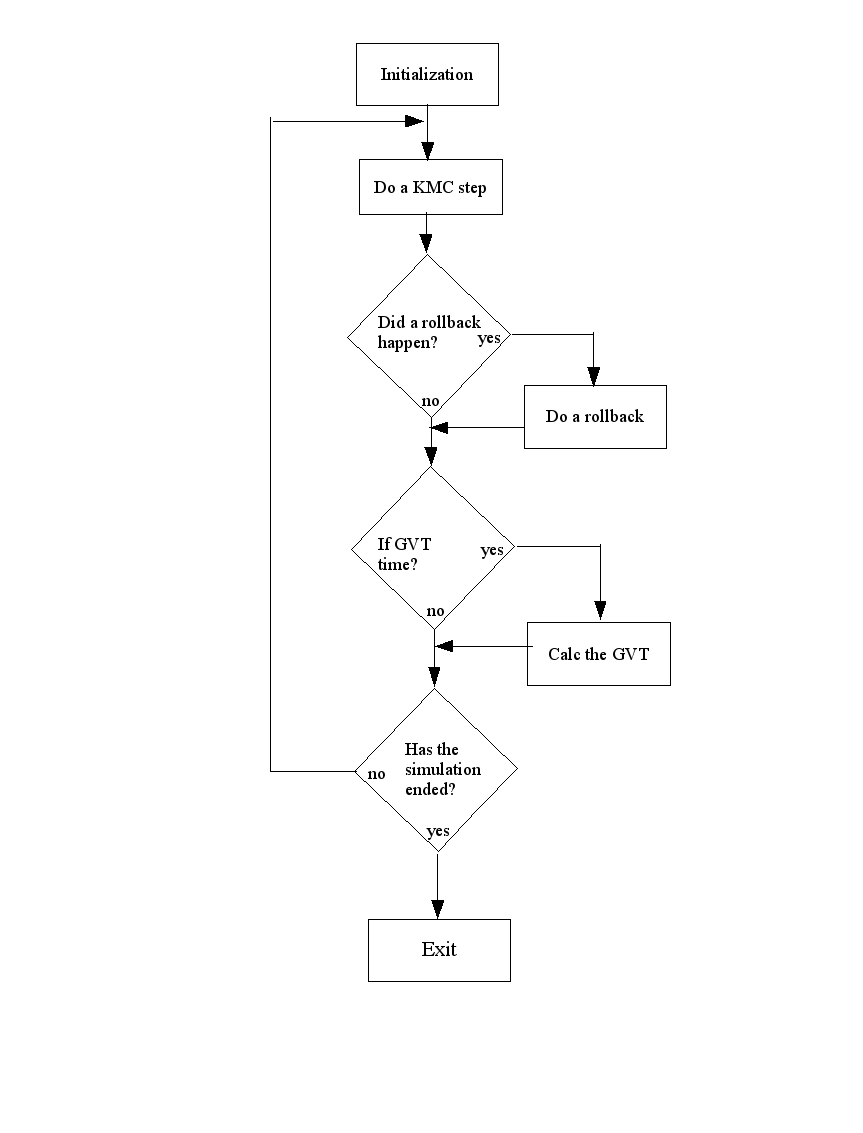
\includegraphics[scale=0.6]{timewarp_flowchart}
\hrule
\caption{Sample KMC Results}
\label{figure:Class Schema}
\end{figure}

The mechanics of the KMC algorithm have already been described in Section \ref{section:Thin Film Growth}.  Since the goal of this project was to delve into the underlying mechanics of the algorithm, of which the KMC was an appropriate problem, the code needed to be written in such a way that it was both flexible and robust.  To facilitate this it was determined that the C++ language would be up to the job.  It was also determined that any of the KMC parts should be as self-contained as possible, which like the re-implementation of SR, was in the form of a Lattice class.  The Lattice class was supported by various layers \ref{figure:Class Schema} of abstraction that removed as much of the implementation dependence as possible.

\section{Implementation}

The actual code base for this implementation of the TW: KMC algorithm is split into an number of files, both C++ source and header files, which contain a number of classes that do nearly all the work.  A text dump of the source files are available in Appendix \ref{ch:Time Warp Code}.

\subsection{Lattice Class}

This sub-section refers to the following appendix sections: \ref{code:tw/lattice.h}, \ref{code:tw/lattice.cpp}, \ref{code:tw/latconst.h}, \ref{code:tw/latprim.h}, \ref{code:tw/rewindlist.h}, \ref{code:tw/randgen.h}, \ref{code:tw/event.h}.

The core of the TW: KMC implementation is a Lattice class.  The design of this class was twofold:  1) To improve on the previous Lattice class as implemented in the new SR code (Appendix \ref{ch:Synchronos Relaxiation Code}) and 2) To build in a new way of handling events that improves the storage and computational efficiency of error correction.

Before the Lattice class proper can be addressed, one must understand the breakdown of the various parts.  In the file \texttt{latprim.h} (Appendix \ref{code:tw/latprim.h}) are the primitive data structures that make up the most atomic parts of an event.  In the file \texttt{event.h} (Appendix \ref{code:tw/event.h}) is the definition of the Event class.  The file \texttt{latconst.h} (Appendix \ref{code:tw/latconst.h}) contains all of the various lattice constants, such as deposition rate and lattice size.  The two support classes, a RewindList abstract data structure (Appendix \ref{code:tw/rewindlist.h}) and a rewindable random number generator (Appendix \ref{code:tw/randgen.h}), are contained in separate files.  The Lattice class is contained in the files \texttt{lattice.h} and \texttt{lattice.cpp} (Appendix \ref{code:tw/lattice.h} and Appendix \ref{code:tw/lattice.cpp}, respectively).

The core of the Lattice class is the event processing.  In previous algorithms, as events are generated they're processed immediately.  Remote events are stored in a buffer and exchanged during a sync.  The same holds true in this implementation, but it is done in a more object-orientated way, where the event becomes an object, and the object is worked upon.

The first that that must be done is determine the locality of the event that must be processed.  Since we're going to be doing error correction using remote events, we must make sure to process events from the remote queue in the correct order.  To do this, we calculate the time of the next local event and compare that value with the earliest event in the remote event queue.  The lowest event is processed.  If it is a local event, we create the event.  For remote events we grab the event out of the queue.

Once we have the event, we proceed to the next step.  This step is to commit the event to the lattice.  At this stage we don't care if it's a remote event or not, and we perform the action, wither deposition or diffusion,  After the event is committed we push it onto a stack of events processed.

Remote events are passed to the communication class, MPIWrapper, during this step as well.  This is a pretty abstract process from the Lattices point-of-view, as all the Lattice needs to know is which boundary the Event occurs on, and what the event is.  The wrapper layer (in this case \texttt{MPIWrapper}) can then translate the passed data and send the event.  The details of this operation in the \texttt{MPIWrapper} layer is covered in Sub-Section \ref{subsection:MPIWrapper Class}.

The Lattice class also needs to check for new remote events.  Currently this is done periodically in the main function, after one event is processed.  This is important, since we must gather the remote events to correct any error we may have made, and to have the events on hand so we don't make an error in the future.  Some though should be put into how often we poll the queue for new remote events.  More often then not, polling once a cycle, we're not going to have any remote events.  However, if we make the polling interval too long, the chances for errors to occur goes up drastically, which means more rollbacks.

The function that polls for remote events is responsible for detecting errors in the simulation as well.  When it finds an error, it will trigger a rollback.  The rollback function takes a single parameter which is the time at which the error occurs.  The rollback function loops through the event stack and compares the top of the stack with the passed timestamp, stopping when the top of the event stack is less-than the passed timestamp.  Each cycle of the loop, if we're not going to halt, the top event is poped off and the event is rolled back on the lattice.  If the event is a remote event, it's stored in the remote event queue, otherwise the event will be discarded.  Sadly, this means that we must send anti-messages for any event that was sent as a boundary event.  Normally this would not be an issue, as the TW algorithm would use lazy evaluation in sending anti-messages, only sending anti-messages for those events that would never happen again.  However, this will be a rare, if not impossible situation, as any KMC event influences the rates for future events, and therefore the probability of that event happening in the same way again.  Since we are almost guaranteed to not repeat the event, we might as well cancel all of the sent events with their anti-message, so we don't need to incur the overhead of lazy evaluation.

The Lattice class would be nearly useless without data output.  There are a variety of ways that one can get data from the Lattice class, including dumps of the height map in both text and as a PNG file.  Also the Lattice and dump it's current monomer list and a collection of various counts and statistics that describe the simulation to that point.  Most of these functions take a output stream as a parameter, with one taking the file name that should be created.

\subsection{MPIWrapper Class} \label{subsection:MPIWrapper Class}
This sub-section refers to the following appendix sections: \ref{code:tw/mpiwrapper.h}, \ref{code:tw/mpiwrapper.cpp}.

The MPIWrapper class is divided into two files, the definition file \texttt{mpiwrapper.h} (Appendix \ref{code:tw/mpiwrapper.h}) and the implementation file \texttt{mpiwrapper.cpp} (Appendix \ref{code:tw/mpiwrapper.cpp}).  Included in these files are any helper structures, such as \texttt{message}.  As the name implies, this class is a wrapper for all of the MPI related calls the program must make.

MPIWrapper provides a number of interfaces for doing various helpful things with MPI.  Included are calls to do global scatter-gather operations and do barrier calls.  The most important interface provided is the sending of events between processes.

The event passing interface is very abstract, compared with previous implementations.  In the original SR code, the MPI calls were performed directly, so the lattice functions needed to know the particulars of the MPI calls and such.  With the MPIWrapper, the Lattice class only needs to pass the event as an Event class pointer and the direction (or boundary) direction as an enumerated integer.  The MPIWrapper call transforms the object as passed into a data structure (type \texttt{message}) which it then can send to the corresponding node.  To mark the type of message, either an event message or anti-message, the tag property of the send call is used.

It should be noted that the send call used in this operation is \texttt{MPI\_Bsend()}, which buffers the message in a local buffer (for this project a 10MB buffer), and only sends the message when the receiving node is ready to receive.  This allows for a asynchronous send, with a blocking receive.

Since the Lattice class must also gather remote events, there is also an interface that returns a list of events as they were received.  There is the possibility that the wrapper could stall out program execution if there are many, many events waiting to be received.  However, this would require a enormous number of events, and in such a situation the current communication model would not be ideal.

The interfaces for sending and receiving anti-messages are the same as the ones provided for normal messages.  The only difference between the function is the tag passed to the MPI calls within.

Also exposed are a suite of function that perform a \texttt{MPI\_Allreduce()}, each function uses a different data type, and takes a data value and a MPI operator as parameters.  This is useful for collecting global statistics and performing the GVT calculation.

Lastly, the MPIWrapper exposes a method to output statistics about it's communications, such as counts of events sent and received and pertinent data about the cluster itself such as number of nodes and who are the neighboring nodes.

\subsection{Main Function and GVT}

This sub-section refers to the following appendix sections: \ref{code:tw/main.cpp}.

The main function of the project is contained in the file \texttt{main.cpp} (Appendix \ref{code:tw/main.cpp}).  Laid out in the main function is the highest level of abstraction in the code, along with the GVT calculation and the calculation of the stopping condition, which is currently the coverage of the lattice.

The level of abstraction in \texttt{main()} is meant to insulate the top level code from the actual processes underneath.  The program is essentially constructed of a main loop that calls a function to process the next event, and then receive and processes any remote events.  Also, at periodic intervals it performs a GVT calculation.  Currently this does nothing as the garbage collection has not been implemented.  The \texttt{main()} function is responsible for outputting the data in various forms along with logging the progress of the simulation for debugging purposes.

The GVT calculation is an all reduce operation that finds the minimum LVT of all the TW objects in the simulation.  This value is set as the GVT.  No event will ever come before this time, so we can effectively delete any data up to that point.  However, this is not done right now.  GVT also makes a decent exit condition for the simulation, is we need not compare the results against previous implementations.

To compare the simulation results against other implementations we need to find the global coverage of the simulation, which requires a second all reduce operation, this time to sum the number of depositions and therefore the number of monomers in the simulation.  To find the coverage we divide the number of monomers by the total surface area of the lattice.  We exit when that value grows greater then 1.0 (100\%).

\section{Issues}

A variety of problems were encountered while implementing the TW algorithm previously described.  Most have been solved, many being bugs with the underlying communication system doing things that more then likely were not intended by the authors.  However, at the time of writing, there has been a bug that shakes the very root of the problem.  Work has stalled out until this bug can be over come.

The bug in question deals with the validity of results obtained at the completion of the simulation.  The results are not consistent from one simulation to the next, which indicates a problem with the rigorous nature of the algorithm.  Normally, the simulation should always, \textit{always}, produce the same results for a given input, baring major hardware failure or a bug (such as the Pentium Floating Point bug) in the actual system hardware.  However, this bug is not a hardware bug, but rather a software bug of the systemic nature.

There could be a variety of causes for such a bug, including a logic error in the error-correction mechanism (rollback) to a race condition.  So far, only a few ideas have been floated, mostly dealing with a race condition between processes to get the first event.  This race condition would then influence the results of the simulation enough to produce drastic results to the final output, as is the nature of the KMC algorithm, one event precipitate further events of random nature.  Logically, however, there are only a few conditions that such a race condition could cause, as there is a limited number of "first events", to start the ensuing chain leading up to the final result.  Suppose that there are $n$ processes, each operating independently of each other.  In the case that thread \#1 were to generate the first event, we would see one result, if the rest of the simulation were truly rigorous.  The same for thread \#2 generating the first event.  It follows that for $n$ processes, we get $n$ results.  This is not observed.

Even if there is not a race condition currently, it may be adding to the problem of debugging the actual cause of the differing results.  A sort of error on-top of an underlying error.  One thing that this implementation discards is the idea of a circular lattice, which is present in the original and rewritten SR algorithms.  The author did not think of the implications of this decision, namely events that happen on the two boundaries that have no neighbors.  In the current TW implementation these messages are just discarded in the wrapper layer.  However, they should be "wrapped around".  This would cause the simulation to disregard the race condition, as it does not matter which process sends or receives the first message since all messages are handled.  The only difference between runs should be the order of the lattices, where the results will be transposed over some number between $0$ and $n-1$ offset from a null state, as the lattice is now a ring, rather then a bar.

It would be more probable that the error occurs during the error-correction sequence.  A logic error in this section of code could precipitate a chain of errors which would end up drastically changing the results.  However, this is a difficult thing to debug, not only because of limitations in the work environment, but because there are many, many events exchanged for a given time period, and it is difficult to sift through them all and make sure all of the events were handled.  This is the next task to tackle and should take a good long time to complete.  Not only will further code need to be written to facilitate this debugging, but then the code will need to be corrected, which in the extreme possibility could necessitate a total rewrite of the error-correction code.  However, this is in the extreme case that it's totally wrong, which isn't very likely.  An educated guess would be that the conditions on the while loops that control the correction are wrong.

It should be noted that both of these conjectures about the possible cause of the current major bug are just that, pure speculation.  Lots of time has been spent on this algorithm, so they are educated guesses, but the root cause could turn out to be something entirely different from the ideas laid out here.  However, once this bug is resolved, there is a good chance that the algorithm is correct and hard performance results can be gathered and future work can take place.